\documentclass{article}
\usepackage{parskip}
\usepackage{graphicx}
\usepackage{caption}
\captionsetup{justification=raggedright, singlelinecheck=false}
\graphicspath{ {./images/} }
\title{Final Report}
\author{By Project Prime}
\begin{document}
 \maketitle
 \section{\underline{Introduction}}
In this project, we were tasked with building a multi-host file synchroniser consisting of three components: a server, a mobile client and desktop client. The server is the \textit{hub} while the clients are the \textit{spokes}. The server was created using Node.js, where it adopted the role of an interface between the clients and MongoDB database. In addition, the server is stored in the Heroku cloud platform to provide both clients with universal file access and processing. The Node.js server can also process HTTP requests to allow both clients to upload, delete and download files. The mobile client was developed using Java and XML on Android Studio, whereas the desktop client was developed using Javascript, HTML and CSS on Electron. The output of the project is a fully-functioning file synchroniser that interacts with both clients via the Node.js server. This project addresses the problem of long durations to complete tasks; thus, the solution will take the form of two clients that minimise the duration to complete tasks as low as possible.
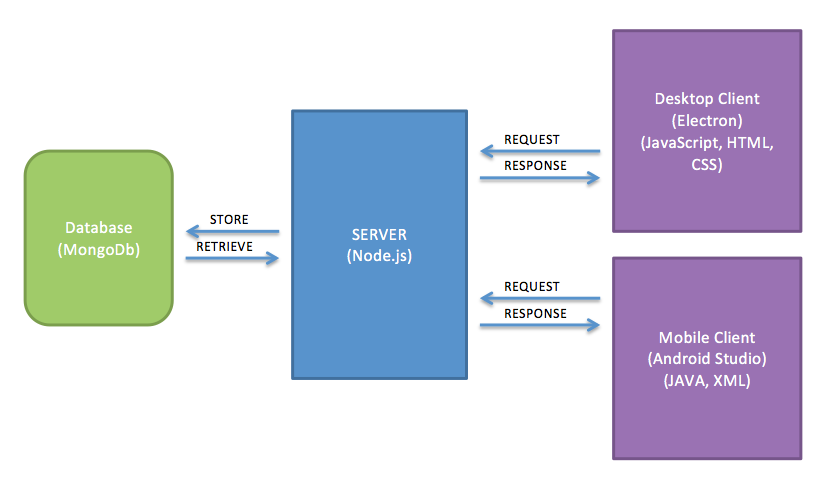
\includegraphics[width=12cm]{/server/serverpic}

\section{\underline{Review}}
\subsection{\underline{Server Application}}
The different techniques which can be used by the the server and client can communicate are...
\begin{itemize}
\item \textbf{XMLHttpRequest:} XMLHttpRequest objects are used to interact with the server. The data can be retrieved from the URL itself. It is heavily used in AJAX programming.
\item \textbf{Server-Sent Events:} SSE is a technology enabling the browser to receive automatic updates from a server by means of HTTP connection.
\item \textbf{WebSocket:} WebSocket is a communication protocol, which provides full duplex communication channel i.e. bi-directional communication between the client and server.
\item \textbf{Hypertext Transfer Protocol (HTTP):} HTTP is a request-response protocol and is stateless. The user initiates requests and the server responds accordingly.

Moving on, according to Jim, Pierce and Vouillon (2002), the connection between client and server can be done in two ways: Socket mode and Tunneling mode. In socket mode, both processes are manually started and the client connects to the server on a predetermined port. In tunneling mode, the client process starts first, it uses SSH to start the server process and communication is conducted using pipes. For example, Unison is more client-oriented which adopts a simple client-server architecture.
\end{itemize}
 
Another application that is commonly used is Dropbox. Dropbox is more server-oriented. According to the Dropbox website (Dropbox Business, n.d), Dropbox possesses different server components...
\begin{itemize}
\item Block servers
\item Metadata servers
\item Storage Servers
\item Paper application servers
\item Paper image servers
\end{itemize}

In our application, the communication is between a server and two clients: desktop and mobile. The clients send a HTTP request to the server and the server responds to the request accordingly. HTTP is a generic stateless protocol. The server recieves the request and responds to the clients with certain results and subsequently, the connection disconnects. So the client and server know about each other during current request and response only. Any kind of media can be sent using HTTP.

\subsection{\underline{Desktop Client}}
The common file hosting service, Dropbox, uses a method which they call “Sync” to keep its files updated across mobile and desktop clients. Its split into two stages: upload and download.
Once a file is uploaded through the server, it is added to their database before other clients are notified of its existence. According to (Koorapati, 2014), the host client does not use a traditional file system directory and allocates a namespace for each user. Their metadata database also known as the Server File Journal stores this information and connects directly to one of Dropbox’s server types: Metadata Server. The actual contents of the file are stored in block data servers. The advantage of having a separate database for the metadata here is that the main contents of the files are less vulnerable to threats because they won’t need to be referenced as often as the metadata for reviewing updates about the files. Furthermore, a good file synchronisation software is defined by how robust its security is and their block data servers are all encrypted using “256-Bit Advanced Encryption Standard” as mentioned in (Dropbox, n.d). 
Therefore, the protocol described in (Koorapati, 2014) for Dropbox’s desktop client is as follows:
\begin{itemize}
\item The upload client commits to the metadata server first to check if there exists a namespace for the file stored in the block server already.
\item For new files, the metadata server would return “need blocks” and the client then directly talks with the block data server to store the new file.
\item The process is repeated and any updates to the file can be checked by only talking to the metadata server.
\item To download a file, the downloading client pings the metadata server to retrieve a list of updates. The Server File journal notifies the client that a new file was added.
\item The download client now contacts the block data server directly to access the new file.
\end{itemize}
This protocol shows that both the desktop client and server application in Dropbox are equally involved in the synchronization process. However, this is not always the case in other software, for example Unison, an open-source file sync.

In (Jim, Pierce and Vouillon, 2002), it is mentioned that “most of Unison’s functionality is concentrated on the client side”. At the start of a process, two roots are specified (to a create a replica) and then the client goes through the following steps:
\begin{itemize}
\item \textbf{Update Detection:} The metadata from older version of the files are compared to their current states and each host is notified whether the contents of the files are changed or not.
\item \textbf{Reconciliation:} The list of changed contents are merged together into a “task list” and used to handle conflicts. A conflict is detected if a path is updated in the replica, whether its descendants have also been updated in the other replica, or the contents in the two replicas are not equal. The task list is then displayed to the user through the UI. 
\item \textbf{Propagation:} The changes in the task list are propagated through both the replicas and the server is then notified about the new contents of the file paths that were updated in the process. 
\end{itemize}
The advantage of having a heavy client-side functionality is robustness. Having less burden on their server increases their crash resistance as indicated in (Jim, Pierce, Vouillon, 2002). 

\subsection{\underline{Mobile Client}}
File synchronization (file sync) is a method of keeping files that are stored in several different physical locations up to date. Cloud and storage vendors often offer software that helps with this process. Recent Studies have shown that file synchronisation has rapidly increased for enterprises/organisations to use the cloud as a means for collaboration. (Bhagwat, 2001) File sync is also commonly used for backup and for mobile access to files. Using a mobile device, you can access the files from anywhere if the user has access to the internet. However, file synching often presents security concerns to enterprises whose employees use consumer-grade applications to access business files. With the use of file synchronisation for public cloud, businesses and organisations are able to utilise their business in lower costs and higher efficiency. (Chiang, 2013) It ensures that the data is kept secure and manages integrity between local storages and the cloud server. However, there are issues that have arisen for example if third parties are able to access the information and the information management crisis. 

There are many existing applications that use file synchronisers. For example FreeFileSync uses a synchronisation software that creates and manages backup copies of all your important files. Instead of copying each file every time, FreeFileSync determines the differences between a source and a target folder and transfers only the minimum amount of data needed. FreeFileSync is a open source Software. Moreover, another example of an app in the market is FileyApp. This app allows you to get all you email attachments in one place and can be available in different platforms such as iphone, ipad and windows. (Otherinbox.com, 2019).  FileyApp has many features for instance, automatically download of attachments, track file versions over emails, get notified of new files and share your files and attachments. With all these features implemented in the app, the user has more options rather than just downloading or opening a file. 

\underline{Send anywhere App}

Send anywhere app is an android application that  is a file sharing that lets you quickly transfer files of any size. In order for this application to work, it needs to be connected via Wifi direct. This application also has other features such as cloud storage service where you can move your files to the cloud once it is uploaded. The files transferred within this app are not stored on any servers and there is no limit ot the files that you can share. 

In conclusion, there are many advantages of having a mobile app for organisations. The Most important being the high performance of user experience and the ease of use for sharing files for business or personal reasons. The ProjectPrime App will be designed in a simple way to make it user friendly, it will have all the features that is required in a file sharing app. This app will be specially designed for users to manage and share files efficiently. With your android application you will be able to save files to the internal storage of the phone as well as upload files to the server when the user is connected to the internet. The functionality, reliability and integrity of ProjectPrime will show the superiority of the application intended for a better user experience. 

\section{\underline{Requirements and Design}}
Requirements have been derived for each component. The requirements have been analysed using the MoSCoW prioritisation technique (Madsen, 2017); as a result, each requirement has been placed into one of the following categories: \textit{Must Have} (critical requirements with the highest priority), \textit{Should Have} (important but unnecessary requirements for the final product), \textit{Could Have} (lowest-priority requirements that would be implemented if time permits) and \textit{Won't Have} (least critical requirements that are unrequired for project success). In addition, the subsections will show the designs that reflect the corresponding component.

\subsection{\underline{Desktop Client}}

\subsubsection{\underline{Requirements for Desktop Client}}
\begin{tabular}{|p{3cm}|p{5cm}|p{4cm}|}
\hline
\multicolumn{3}{|c|}{\textbf{MoSCoW requirements for The Desktop Client}} \\
\hline
\textbf{Requirement No.} & \textbf{Requirement} & \textbf{Priority}\\
\hline
1 & Must be able to communicate with the Server Application & Must Have \\
\hline
2 & Has to be able to upload files & Must Have \\
\hline
3 & Has to be able to download files from database via server & Must Have \\
\hline
4 & Make use of a file management system to upload any file from the user's system & Must Have \\
\hline
5 & Check for updates regularly so that the desktop client is in sync with the Server and Mobile Client & Must Have\\
\hline
6 & Display the current list of files from the database in the centre of the page & Should Have \\
\hline
7 & Include a delete file functionality   & Should Have \\
\hline
8 & Provide a way to track and check recent changes to files & Could Have\\
\hline
9 & Include a search bar to quickly find files if the list of files is too large & Could Have \\
\hline
10 & Have User profiles for personalised access & Won't Have \\
\hline
\end{tabular}

\subsubsection{\underline{Designs for Desktop Client}}

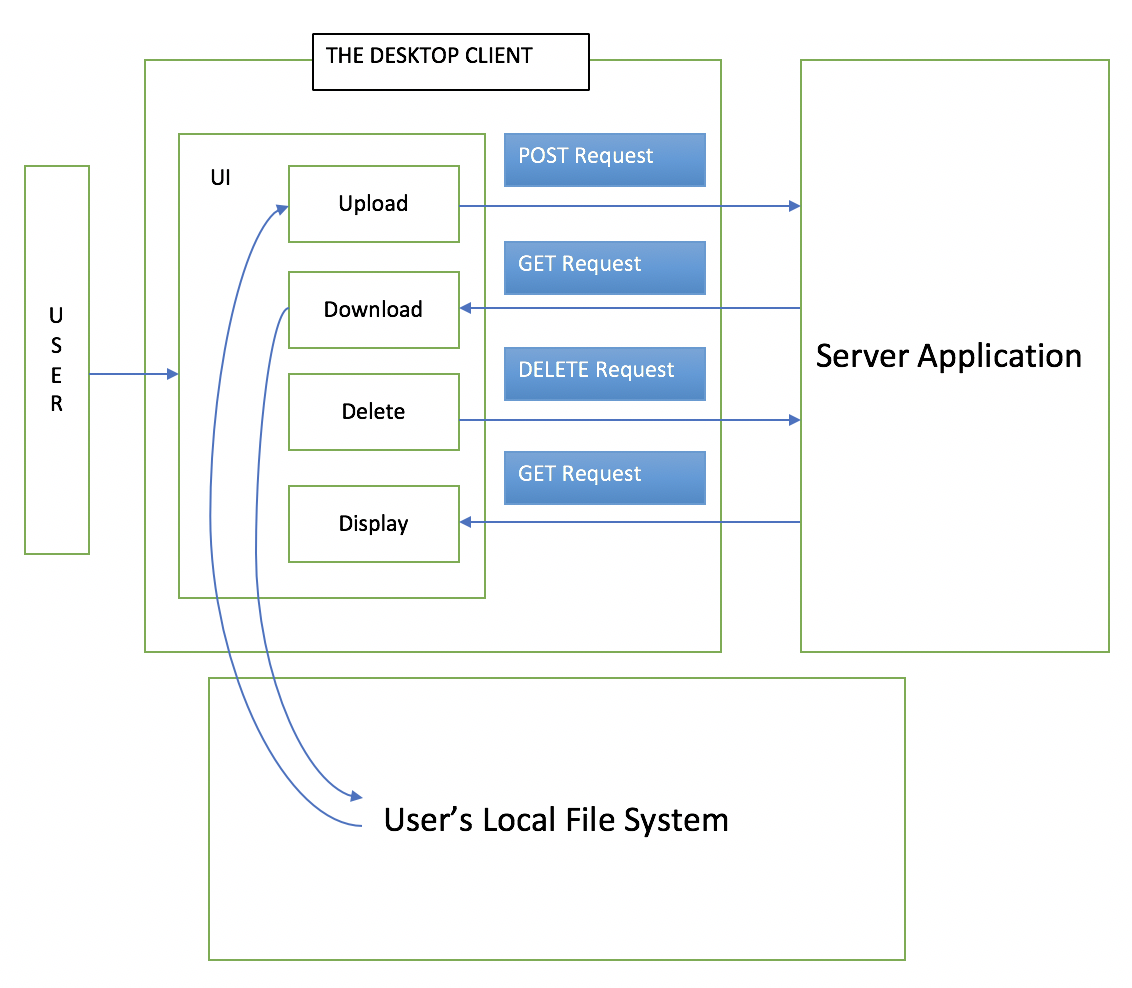
\includegraphics[width=12.1cm]{/design/desktop/architecture}

Above is an architectural diagram of the desktop client. After analysing the requirements, the main functionalities chosen were \textit{Upload}, \textit{Download}, \textit{Delete} and \textit{Display}. The rationale behind this was wanting to focus on the core functionalities to ensure the working client could be tested with the server.

The user will interact with the client through the UI containing three buttons: upload, download and delete. In addition, they will view the files in the server as a list. Interacting with the upload button would access the user’s local filesystem and allow them to select any type of file. Once a file is selected, the client will send a POST request to the server asking it to store the file. The Download button sends a GET Request to the server asking for the specific file to be retrieved and opens the user’s local filesystem to save the file. Delete simply sends a DELETE request to the server asking it to remove the file from the database.

The Display functionality displays all the files in the system by sending a GET request to the server. This allows the user to check for any changes to the metadata such as the filename or any additions/ deletions of files.

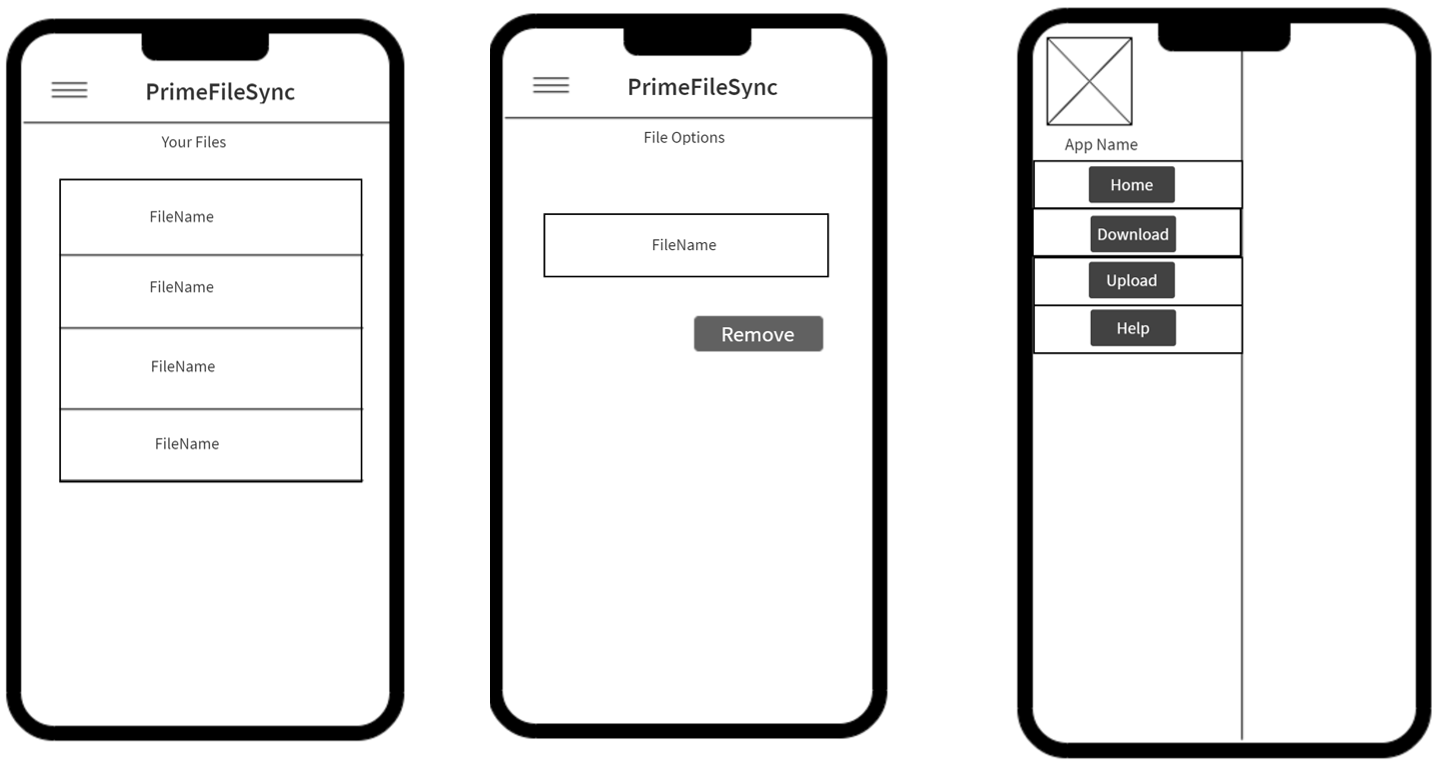
\includegraphics[width=9cm]{/design/desktop/UI}

Following the design philosophy, the above mock UI was sketched using MockFlow. This sketch provided a prediction of the client's appearence.

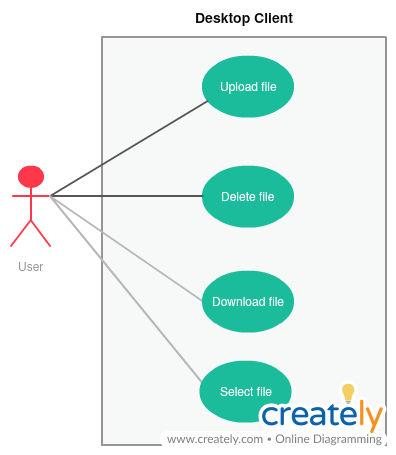
\includegraphics[width=8cm]{/design/desktop/UseCase}

Working under the design philosophy, above is the use-case diagram of the desktop client, which entails the client's functionalities: allowing users to select, upload, delete and download files.

\subsection{\underline{Mobile Client}}
\begin{tabular}{|p{3cm}|p{5cm}|p{4cm}|}
\hline
\multicolumn{3}{|c|}{\textbf{MoSCoW requirements for The Mobile Client}} \\
\hline
\textbf{Requirement No.} & \textbf{Requirement} & \textbf{Priority}\\
\hline
1 & Must be able to communicate with the Server Application & Must Have \\
\hline
2 & Must be able to upload files into the database through the server & Must Have \\
\hline
3 & Must be able to delete files & Must Have \\
\hline
4 & All changes must be reflected in the files stored in the server & Must Have \\
\hline
5 & The mobile UI must be simple and easy to navigate through & Should Have \\
\hline
6 & All the application's functions should be accessible from the main page & Should Have \\
\hline
7 & All files files should be listed with both filename and time of last modification clearly visible to the user & Should Have \\
\hline
8 & Include a search bar to quickly search through the list of files & Could Have \\
\hline
\end{tabular}

\subsection{\underline{Server Application}}

\begin{tabular}{|p{3cm}|p{5cm}|p{4cm}|}
\hline
\multicolumn{3}{|c|}{\textbf{MoSCoW requirements for Server Application}} \\
\hline
\textbf{Requirement No.} & \textbf{Requirement} & \textbf{Priority}\\
\hline
1 & Has to be connected to a database in order to store and retrieve files & Must Have \\
\hline
2 & Must be able to communicate with the Desktop and Mobile Clients simultaneously & Must Have \\
\hline
3 & Use HTTP requests to send data to the clients & Must Have \\
\hline
4 & Handle conflicts using Rsync & Should Have \\
\hline
5 & Use security encryption to protect the data & Could Have\\
\hline
\end{tabular}

The server was created using Node.js. The server waits for client requests and responds to them; thus, providing a service upon their request. It is responsible for handling requests, responding to them appropriately, as well as for establishing and maintaining the database connection.  We decided to use Node.js to build the server as it allows simple writing and maintenance of JS-based backend servers with easy-to-use APIs by the clients. Furthermore, we have used a flexible Node application framework called Express, which creates the middleware and helps to manage everything from routes to handling requests. To store and retrieve files we decided to use a NoSQL database - MongoDB. Unlike a relational database where data is stored in rows and columns, MongoDB stores BSON documents in collections with dynamic schemas.

\begin{figure}[h!]
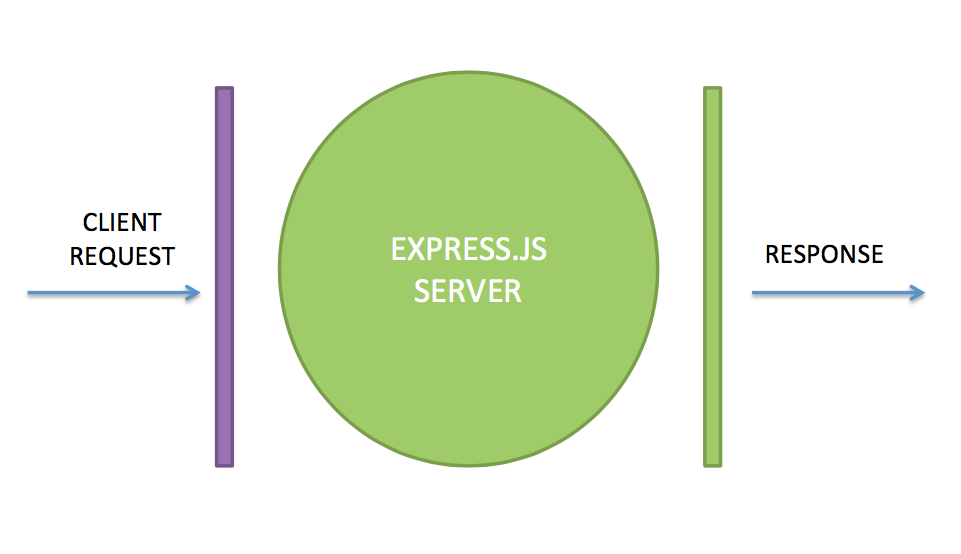
\includegraphics[width=12cm]{/server/expresspic}
\captionsetup{justification=centering}
\caption{Middleware}
\end{figure}

\section{\underline{Implementation}}
\subsection{\underline{Server Application}}
The server was developed using Node.js and the database used is a cloud service by MongoDB. The Node.js server is stored in the Heroku cloud platform.

In table 1, the following packages were used for implementing the server application... 
\begin{table}[h!]
\begin {center}
\captionsetup{justification=centering}
\caption{List of packages used}
\begin{tabular}{l|l}
\hline
\textbf{Package Name} & \textbf{Description}\\
\hline
multer & Used for uploads\\
mongoose & Used to connect to database\\
method-overide & To make a delete request without making an AJAX call\\
\end{tabular}
\end{center}
\end{table}

In table 2, the following API calls were also used in the implementation of the server...
\begin{table}[h!]
\begin {center}
\captionsetup{justification=centering}
\caption{API calls to the server}
\begin{tabular}{l|c|r}
\hline
\textbf{Name} & \textbf{URL} & \textbf{Description}\\
\hline
Display(GET) & (/files) & Returns all files in the database\\
Upload(POST) & (/upload) & Uploads a file to database\\
Download(GET) & (/download/:filename) & Downloads the requested file from the database\\
Delete & (/files/:filename)  & Deletes the requested file from database.\\
\end{tabular}
\end{center}
\end{table}

\begin{tabular}{|p{2cm}|p{2cm}|p{3cm}|p{3cm}|p{3cm}|}
\hline
\multicolumn{5}{|c|}{\textbf{Test Cases for Server Application}} \\
\hline
\textbf{Test ID} & \textbf{Test Name} & \textbf{Expected} & \textbf{Actual} & \textbf{Pass/Fail/Solved} \\
\hline
1 & ... & ... & ... & ... \\
\hline
\end{tabular}

\subsection{\underline{Desktop Client}}
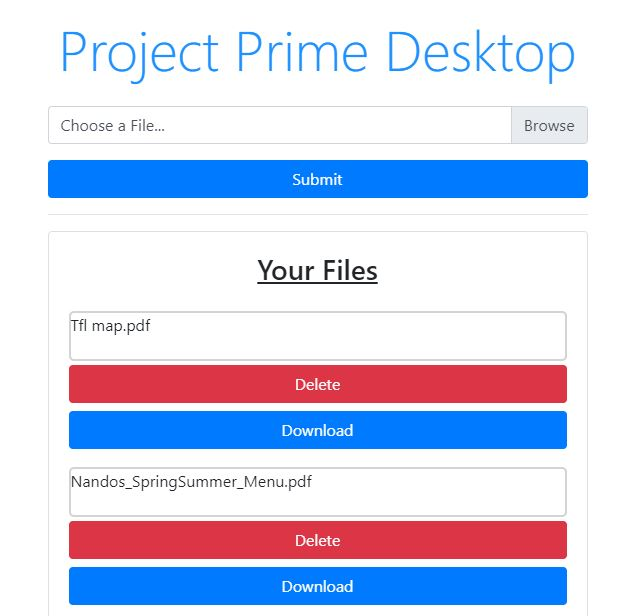
\includegraphics[width=12cm]{/fragments/desktop/frontEnd}

The desktop client was developed using  HTML, Javascript and CSS on Electron. Electron provides pre-written HTML code (Electron, n.d.) that creates a basic desktop app; the pre-written code was used as the foundation for the development of the desktop client. Afterwards, the client's front-end was modified using JS, HTML and CSS to reflect the project designs. On to the desktop client's front-end, Bootstrap CSS files and JS scripts (Bootstrap, n.d.) were also included to add and format certain elements (e.g. file upload bar and button), along with CSS files written by the desktop subgroup.
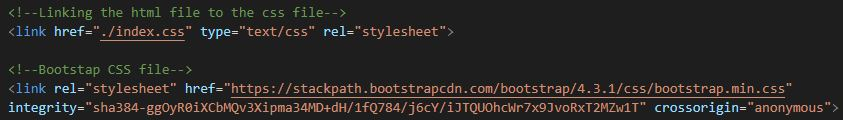
\includegraphics[width=12cm, height=2cm]{/fragments/desktop/BootstrapCSSfiles}

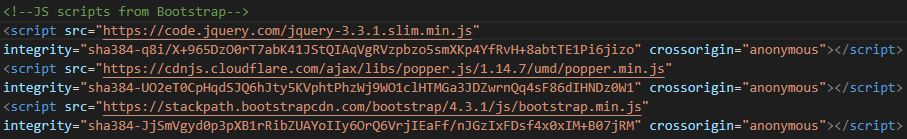
\includegraphics[width=12cm, height=2cm]{/fragments/desktop/BootstrapJSscripts}

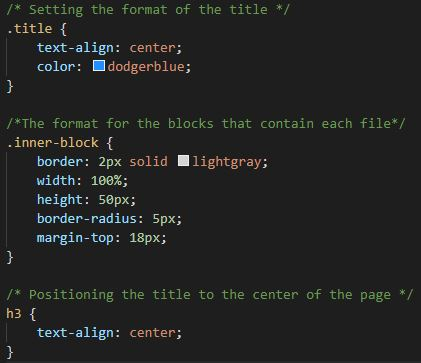
\includegraphics[width=8cm, height=6cm]{/fragments/desktop/css}

After setting the foundation, the desktop subgroup concentrated on displaying files that resided in the database. To do so, the server would return a JSON object (which contains each file in the database) after a connection was formed between the desktop client and server. Using a loop, the object was traversed through and for every file encountered, that file would be presented on the client's UI. In addition, each file would be encapsulated in a file container (presented as a grey-bordered box).

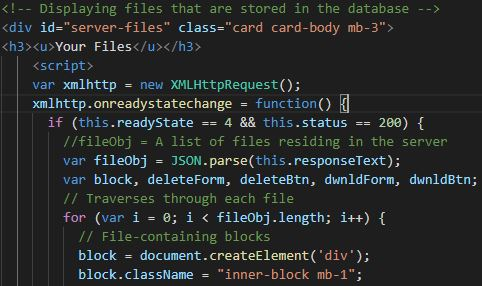
\includegraphics[width=12cm]{/fragments/desktop/display1}

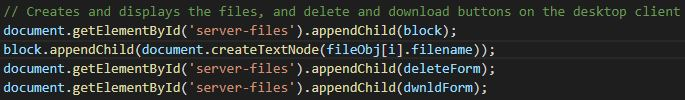
\includegraphics[width=12cm]{/fragments/desktop/display2}

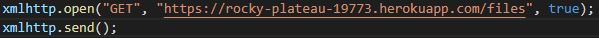
\includegraphics[width=12cm]{/fragments/desktop/display3}

Next, the subgroup wrote code that enabled the client to upload files into the database via the server. After pressing the \textit{Browse} button, the local host's file manager opens, which enables the user to choose a file and subsequently, the label of the file upload bar changes to the name of the selected file; therefore, indicating which file was selected by the user. Afterwards, the user would press the \textit{Submit} button which transmits a http post request to the server, which causes the latter to store the selected file inside the database. In addition, the label of the file upload bar will revert to its initial form (i.e. "Choose a File...") after the \textit{Submit} button is pressed. 

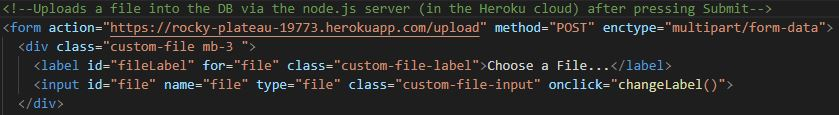
\includegraphics[width=12cm]{/fragments/desktop/upload}

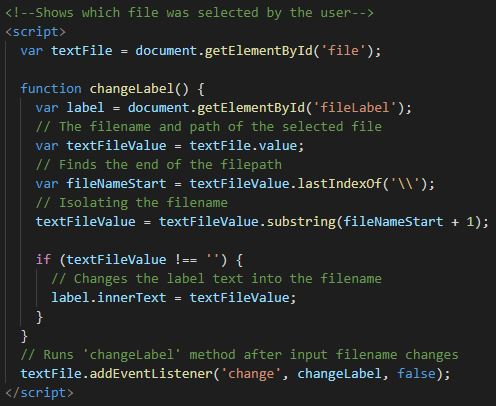
\includegraphics[width=12cm]{/fragments/desktop/upload2}

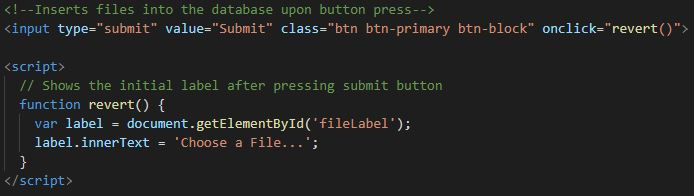
\includegraphics[width=12cm]{/fragments/desktop/upload3}

Moving on to file deletion, the desktop subgroup wrote code that enabled the client to delete files; as a result, removing the corresponding document from the database. To add to this, deleting a file resulted in removing that file from the list of documents displayed on the client's UI. After pressing the \textit{Delete} button, the client would send a delete request to the server and this request would include the file's unique ID; therefore, the use of unique identification ensures the prevention of multiple files of the same name being deleted, for example. 

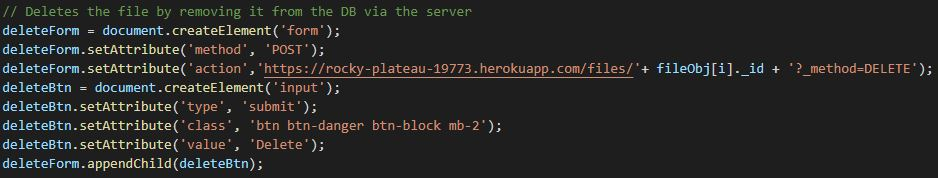
\includegraphics[width=12cm]{/fragments/desktop/delete}

Finally, the desktop subgroup wrote code that enabled the client to download files from the database; as a result, bringing the corresponding document into the storage of the local host. After pressing the \textit{Download} button, the client sends a GET request to the server, which causes the server to return the file in the local host's file manager and the user stores the file in the local host's storage by pressing the \textit{save} button of the file manager. 

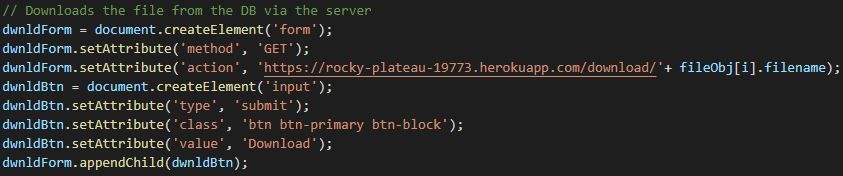
\includegraphics[width=12cm]{/fragments/desktop/download}

\begin{tabular}{|p{2cm}|p{2cm}|p{3cm}|p{3cm}|p{3cm}|}
\hline
\multicolumn{5}{|c|}{\textbf{Test Cases for Desktop Client}} \\
\hline
\textbf{Test ID} & \textbf{Test Name} & \textbf{Expected} & \textbf{Actual} & \textbf{Pass/Fail/Solved} \\
\hline
1 & Connection to server & A JSON object will be returned to indicate the connection between the server and client.  & As expected & PASS \\
\hline
2 & Display file(s) & Display files stored in the Mongo database. & As expected & PASS \\
\hline
3 & Upload file & A file gets uploaded into the database via server after pressing the \textit{Submit} button. Next, the file is displayed in the list of documents stored in the server. & File was uploaded but does not appear in the list unless the page is refreshed. & 1/2 \\
\hline
4 & Delete file & A file gets removed from the database via server after pressing \textit{Delete} button. Next, the list of documents is displayed without the deleted file. & File was deleted but isn't removed from the list unless the page is refreshed. & 1/2 \\
\hline
5 & Download file & A file gets downloaded into the local host after pressing the \textit{Download} button. & As expected & PASS \\
\hline
\end{tabular}

\subsection{\underline{Mobile Client}}
Android studio was used to develop the android application. Android studio is an IDE designed and developed specifically for android app development. Also with a use of a gradle based build system you have the option to preview a layout on multiple screen configurations while editing. With the use of extensible Mark-up Language (XML) it aided the development of the screen layouts. This was beneficial as it gave the ability to meet the usability and functional requirements of the application. To display the screens an android emulator was used, and an android phone was used to make sure the application was running successfully as well as provide a visual feel on how the app would feel.

Nodejs was used to connect the android app to the server. Node.js is an open-source and cross-platform JavaScript runtime environment. To connect to the server numerous methods were used, one being the Android volley library. This library was used because it is an HTTP library that makes networking for Android apps easier and most importantly faster. Android Volley allowed us to do automatic scheduling of network requests and helped support for request prioritisation.  Furthermore, using Android Volley, we...
\begin{itemize}
\item Sent a simple request using the default actions of Volley
\item Set up RequestQueue
\item Made a standard request to send a request using one of Volley's out-of-the-box request types (raw strings, images, and JSON)
\end{itemize}

\underline{Design and Implementation}

The User Experience was very important in the design of this application, so this aspect of the application was carefully considered. The navigation around the application was simple enough for the user to understand. It was decided that the application should follow a consistent design throughout, this meant determining a suitable colour scheme which will be used in all the pages of the application. A navigation menu is used for simplicity reasons to save space on the pages of the application. In the application there are 3 main sections: homepage, file options page and help page. 

\underline{Permissions and Dependencies}
To implement the features of this application, some permissions had to be changed and libraries had to be added. In terms of permissions, we had to add three new permissions into the manifest. 

\begin{itemize}
\item INTERNET : This allows the application to connect to the internet.
\item WRITE EXTERNAL STORAGE: This allows the application to write to external storage.
\item READ EXTERNAL STORAGE : This allows the application to read from the external storage.
\end{itemize}

We also had to add 2 dependencies 

\begin{itemize}
\item Android Volley v1.1.0 : This library was used in the Home Fragment in the retrieval of the files
\item OkHttp v3.3.1 : This library was used in the Home Fragment to upload new files
\end{itemize}

\underline{Home Page}

The home page consists of two main parts including a list which represents all the files and an upload button. To be able to achieve a working list view, we needed to design the layout of each entry of the list, and to code a custom adapter to fill the list view with the data received from the server. The code for the list uses the Android Volley library to send a GET request to the server to request for a JSON response. This response was then separated into 2 Array Lists, chosen due to the simplicity of adding and removing elements. The contents of each of these Array Lists were then copied to 2 String arrays, which were passed to a custom adapter. 

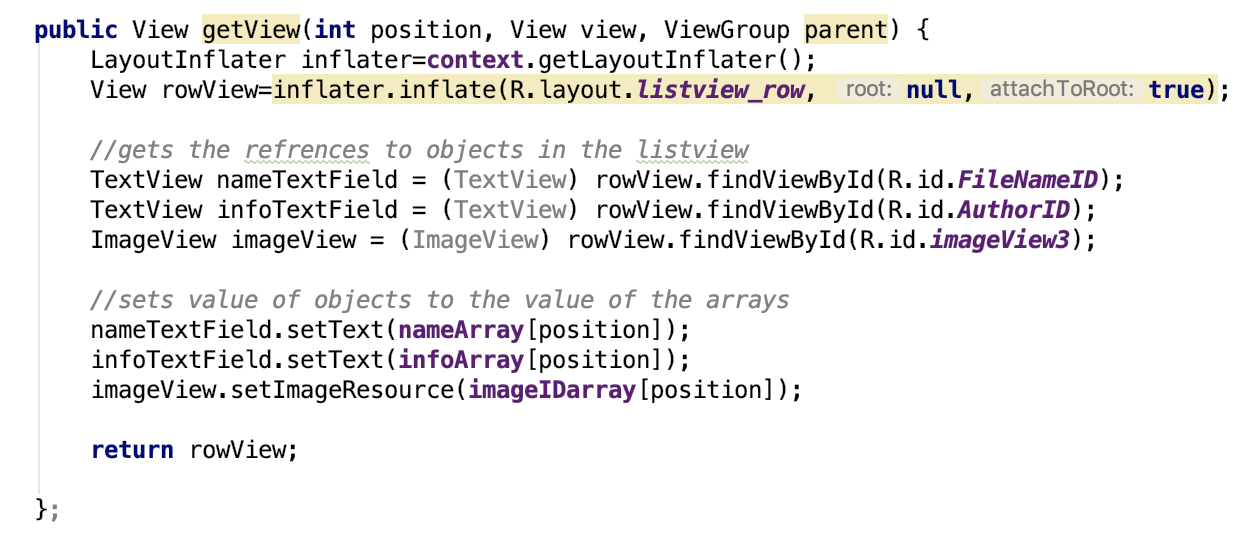
\includegraphics[width=12cm]{/fragments/mobile/adapter}

This custom adapter takes the data passed and assigns it to the correct parts of the list view. Lastly, an 'onclick' listener was used for each entry of the list view to enable the user to access the file options for the file selected. 

The next part is the Upload button, an 'onclick' listener is used for when the user clicks the button, this opens a popup menu which allows the user to navigate the local folder of the device. Android has a library which we were able to use which enabled quick and easy navigation and selection of files in numerous locations such as camera, recent, download and others. 

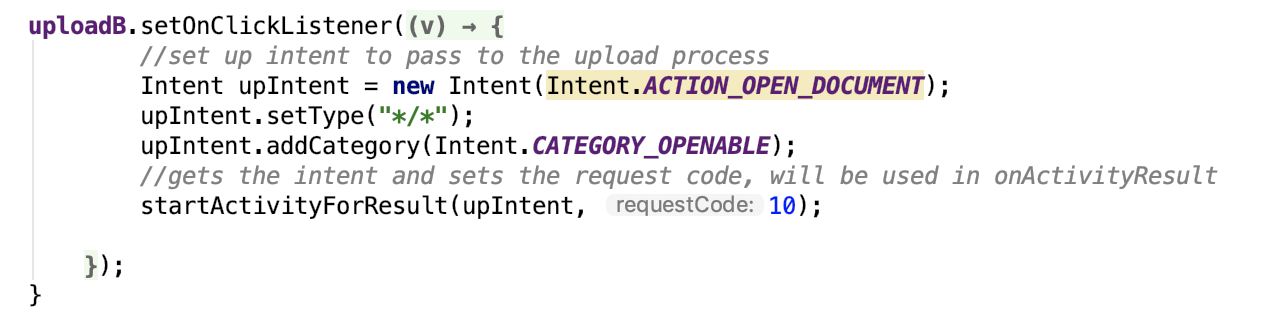
\includegraphics[width=12cm]{/fragments/mobile/uploadbtn}

When a file is selected the Intent and a request code of 10 is passed using 'startActivityForResult()', which triggers the onActivityResult method. Within this method we see that a progress dialog has been started so that the user is aware that an upload is in progress, a new thread is started for the upload request so that the request is not sent on the main thread. In this new thread, the file name and path of the file are obtained by retrieving the URI from the data sent to the method. After getting the file name and file path, an OkHttpClient object is created to send the request. 

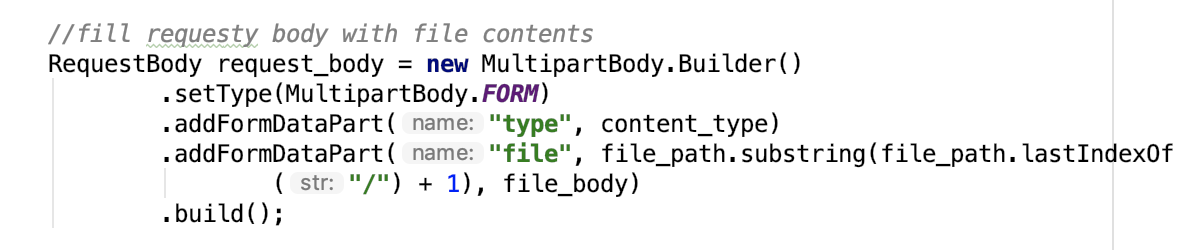
\includegraphics[width=12cm]{/fragments/mobile/builder}

This is created using a MultipartBody builder which prepares the requests body containing the selected files contents. Following this, a request is sent to the target URL with a POST method containing the request body created. If there are no errors the file should be uploaded and the Home Fragment is called again, to display the new file in the list view. 


\underline{File Options page}

When a file has been selected from the list view on the home page, a new fragment is called which will display the name of the file and two buttons ‘remove’ and ‘download’. Firstly, when the Remove button is clicked, an asynchronous task called RemoveFileTask is executed. 

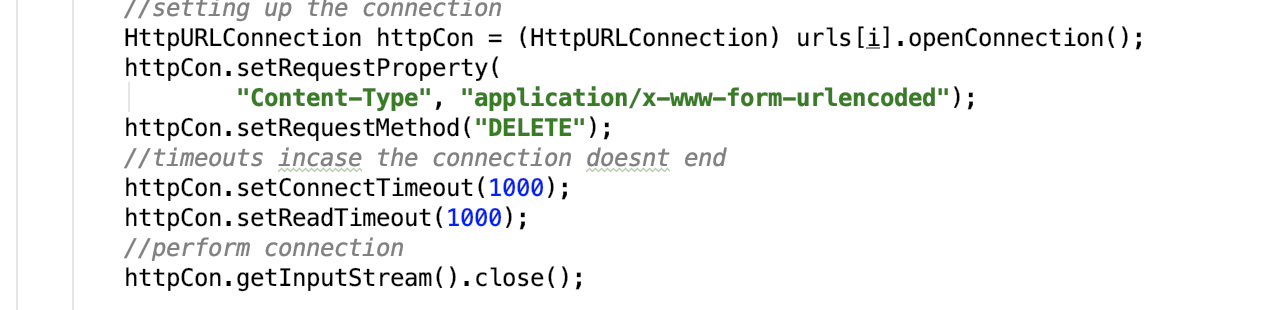
\includegraphics[width=12cm]{/fragments/mobile/deletecode}

This will take the name of the file, which was sent between the home and file options fragment and create an HTML delete request which is then sent to the server. This is done using an httpURLConnection with request method ‘DELETE’. This code is done as an asynchronous task as having this run in the main thread would cause a UI crash. 

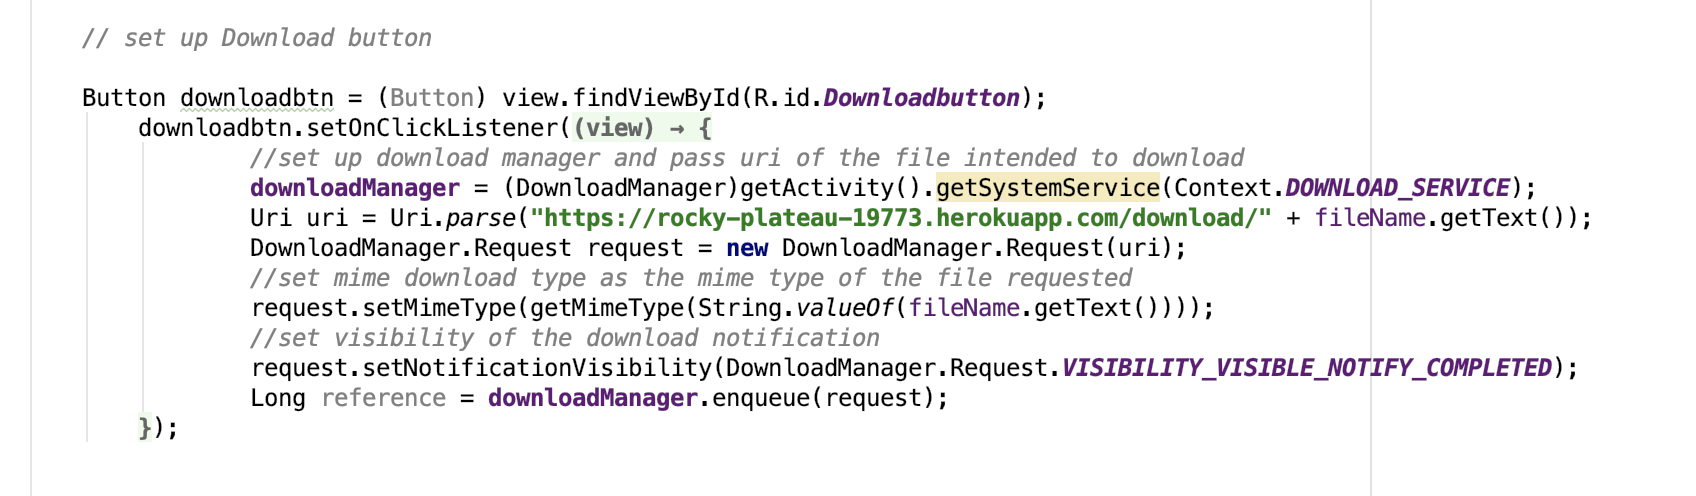
\includegraphics[width=12cm]{/fragments/mobile/downloadbtn}

Secondly, the download button on the file options page uses the android predefined class DownloadManager to request a file from the server. To ensure that it downloads the file with the correct MIME type, the request has to be set to the MIME type of the file requested, to do this a check MIME type method is used to retrieve this information. A setNotificationVisibility is also set to alert the user when the download is in progress and when it is complete. This request is then added do the downloadManager queue. 

\underline{Help Page}

This page contains text which will provide information to the user on how the application works.  


\begin{tabular}{|p{2cm}|p{2cm}|p{3cm}|p{3cm}|p{3cm}|}
\hline
\multicolumn{5}{|c|}{\textbf{Test Cases for Mobile Client}} \\
\hline
\textbf{Test ID} & \textbf{Test Name} & \textbf{Expected} & \textbf{Actual} & \textbf{Pass/Fail/Solved} \\
\hline
1 & Get list of files from server & List view would show all files on the server & As expected & Pass \\
\hline
2 & Smooth and efficient navigation between pages & All pages can be accessed through the app with smooth transitions & As expected  & Pass \\
\hline
3 & Clicking on file in list view & file options fragment opens with selected file name shown and remove and download buttons & As expected  & Pass \\
\hline
4 & Download button (File options page) & Pressing download will result in only downloading the file selected to the device & As expected  & Pass \\
\hline
5 & Remove button pt.1 (File options page) & Pressing Remove will result in removing only the file selected from the server & The file is removed, however the connection fails to terminate on its own, a timeout is used to end the connection after given enough time to complete the request & Solved  \\
\hline
6 & Remove button pt.2 (File options page) & After the file is removed, the user is sent straight back to the Home page where the file list view can be seen & After the request is sent, the UI is changed back to the Home page, however the UI changes faster than the server processes the request, a thread.delay() is used to slow down the UI change to give the server enough time.   & Solved \\
\hline
7 & Upload button (Home page) & Pressing upload will result in opening a file selection window, once a file is selected only the file selected will be uploaded to the server, & As expected  & Pass \\
\hline

\end{tabular}

\section{\underline{Teamwork}}
Project Prime consists of six members: Yusaf, Sandipan, Saloni, Shefali, Cameron and Manny. To balance the workload, the team was divided into three subgroups of two teammates and each subgroup was assigned to the development of one component. As a result, Yusaf and Sandipan were assigned to the desktop client, Saloni and Shefali were assigned to the server, and Manny and Cameron were assigned to the mobile client. Within these subgroups, the work was distributed between both teammates through discussion. Despite the team division, members from other subgroups were permitted to intervene in the development of a component that they weren't assigned to, in order to fix issues that the assigned subgroup couldn't correct, for example. Moving onto communication, the team remotely communicated using an instant messaging app (i.e. Whatsapp), which allowed arrangements of group sessions at a certain date-and-time, notifying teammates of open pull requests, etc. Furthermore, the sessions were conducted in booked study rooms at least once per week and these sessions involved group discussion and coding of all components. Next, the project involved Github, where the project implementation was contained in a public repository called \textit{Project Prime Dev}. In addition to Git, the team followed the feature branch workflow, where a component feature was developed inside a branch seperate to the master branch and subsequently, the former would be merged into the latter branch.

\section{\underline{Evaluation}}
To start with what went well, one positive aspect was the firm strength of team communication, as all members proactively shared their thoughts and concerns in physical meetings and in the WhatsApp group. In addition, communication was carried-out in a respectful manner at all times; thus, there were no verbal conflicts during the project. Another positive aspect was the fairness in workload distribution by creating subgroups that were assigned to the development of a specific component. The rationale behind the formation of subgroups was to avoid the possibility of one member feeling overwhelmed from having lots of work. Furthermore, by assembling subgroups, this influenced the members of the subgroup to cooperate together to build the component; thus, being in a subgroup generated a sense of teamwork. Finally, a notable positive aspect was our ability to adapt to changing circumstances. For instance, it was initially planned to store files in a SQL database. Unfortunately, we discovered SQL databases were unideal for file storage since it is limited by file size. In response, we decided to migrate to MongoDB, which is a cloud service that allows the creation of document-oriented database systems that can contain files of any size.

\noindent Moving on to what didn't go well, our initial plan was weak as we didn't know how to approach the task, due to having no experience in developing file synchronisers. Although we met various project objectives, our commitment to the plan was low, as we rarely compared our progress to the initial plan during our weekly meetings. Another negative was the poor interactive feedback of certain features in particular components. For example, after pressing the \textit{Browse} button in the desktop application, there is no feedback (e.g. temporary colour change, mouse cursor change) to indicate the button-pressed.

\noindent Relative to the initial plan, there were differences between the rough timetable and actual progress. For instance, instead of using an SQL database, we decided to create and use a MongoDB database since it's document-oriented and has the capability to store files of any size, whereas SQL storage is limited by data type and size, and it cannot process text files properly; thus, with MongoDB being more suited to our needs, we abandoned the plan to use an SQL database and shifted to MongoDB instead. Another difference was the additional design work conducted, since as initially planned, the clients were going to only be sketched. However, to support the implementation of both clients, we decided to create use-case and architectural diagrams to know the core functionalities to build and to understand the structure of both systems, respectively.

\noindent There were several cases where the project experienced change that was forced upon us or was the result of improved thinking. An example of the latter, the server was formerly stored in a laptop owned by a teammate, whom was part of the server subgroup. However, the server's IP address changed based-on the laptop's current location; therefore, locally storing the server resulted in constantly changing the server's IP address within the clients' source code. This proved to be a tedious task throughout the progression of the project. As a solution, we decided to store and run the server on Heroku, which is a platform-as-a-service (PaaS) that enables applications to operate on the cloud; thus, this removed the tediousness of changing the server's IP address in the source code of each client.  

\noindent On to how the team worked together, the team was divided into three subgroups as initially planned, where each subgroup developed one component of the file synchronising system; as a result, the workload was divided fairly amongst all members. Throughout the majority of the project's lifetime, the team attended group meetings once per week where group discussion and coding was conducted. Along with group meetings, communication was also conducted in a whatsapp group where we scheduled groups meetings in booked study rooms at a certain date-and-time, notified each other about opened pull requests, reminders about incomplete work, etc. The reason for choosing whatsapp as our main form of remote communication was due to everyone's familiarity with the app and its simplicity (in terms of usability); thus, there was no need to use Skype since the team was comfortable with using whatsapp, in contrary to the original plan. Despite developing the system outside the meetings, one major weakness was scheduling meetings once per week since it delayed the completion of work, which could have been completed faster if we met more than once per week by completing tasks together. Overall, the team worked well together, as there were no conflicts and each member contributed their unique  skills to the group. For instance, since Yusaf possessed leadership experience, he was elected as team leader to command the group, ensure each member's involvement in the project's activities, etc.

\noindent In conclusion, this project caused the realisation that despite our computer science backgrounds, our technical prowess is still very basic and there is much for us to learn. In response to this discovery, we will commit to thoroughly relearning and practising how to use different technologies in our spare time, including programming languages and Git (e.g. BitBucket). In retrospect, if this project was repeated, our different approach would be to partner stronger members with novice ones, in terms of technological skill; thus, providing novice members with the opportunity to enhance their skills by learning whilst working on the job.   

\section{\underline{Peer Assessment}}
\begin{tabular}{|p{1.5cm}|p{1.5cm}|p{1.5cm}|p{1.5cm}|p{1.5cm}|p{1.5cm}|}
\hline
\multicolumn{6}{|c|}{\textbf{Peer Assessment of Project Prime}} \\
\hline
\textbf{Yusaf} & \textbf{Sandipan} & \textbf{Saloni} & \textbf{Shefali} & \textbf{Cameron} & \textbf{Manny} \\
\hline
17.5 & 16.5 & 16.5 & 16.5 & 16.5 & 16.5 \\
\hline
\end{tabular}
	
\section{\underline{Bibliography}}
\begin{tabular}{|p{12.2cm}|}
\hline
\multicolumn{1}{|c|}{\textbf{Reference List}} \\
\hline
Bootstrap (n.d.) \textit{Introduction} [online] Available at: https://getbootstrap.com/docs/4.3/getting-started/introduction/ [Accessed on 25th March] \\
\hline
Dropbox Business. (n.d) \textit{Under the hood: Architecture Overview} [online] Available at: https://www.dropbox.com/business/trust/security/architecture [Accessed on 17th March] \\
\hline
Electron (n.d.) \textit{Writing your First Electron App | Electron} [online] Available at: https://electronjs.org/docs/tutorial/first-app [Accessed on 12 March 2019] \\
\hline
Madsen, S. (2017) \textit{How to Prioritize with the MoSCoW Technique} [online] Available at: https://www.projectmanager.com/training/prioritize-moscow-technique [Accessed on 10 March 2019] \\
\hline
Nipuun Koorpati. (2014) \textit{Streaming File Synchronization } [online] Available at: https://blogs.dropbox.com/tech/2014/07/streaming-file-synchronization/ [Accessed on 17th March] \\
\hline 
Jim, T., Pierce, B., Vouillon, J.  (2002) \textit{How to build a File Synchronizer} [online] Available at: http://web.mit.edu/6.033/2005/wwwdocs/papers/unisonimpl.pdf [Accessed on 26th March] \\
\hline
Chiang, J.K., 2013. Authentication, Authorization and File Synchronization for Hybrid Cloud-The Development Centric to Google Apps, Hadoop and Linux Local Hosts. \\
\hline
Send-anywhere.com. (2019). Send Anywhere. [online] Available at: https://send-anywhere.com [Accessed 24 Mar. 2019]. \\
\hline
 Bhagwat, P., 2001. Bluetooth: technology for short-range wireless apps. IEEE Internet Computing, 5(3), pp.96-103. \\
\hline
Otherinbox.com. (2019). Filey | OtherInbox, the App Store for Email. [online] Available at: https://www.otherinbox.com/filey/ [Accessed 26 Mar. 2019]. \\
\hline
\end{tabular}
\end{document}